\documentclass[12pt,letterpaper]{report}
\usepackage[margin=1in]{geometry}
\usepackage{titlesec}
\usepackage{amsmath}
\usepackage{amssymb}
\usepackage[colorlinks=true,urlcolor=black,linkcolor=black]{hyperref}
\usepackage{graphicx}
\usepackage{biblatex}
\usepackage{textcomp}
% extra packages you need
\usepackage{graphicx}
\usepackage{listings}
\usepackage{algorithm}
\usepackage{algorithmic}
\usepackage{amsmath}
\usepackage{latexsym}
\usepackage{amsfonts}
\usepackage[normalem]{ulem}
\usepackage{array}
\usepackage{amssymb}
\usepackage{subfig}
\usepackage{wrapfig}
\usepackage{wasysym}
\usepackage{enumitem}
\setlist[itemize]{after=\vspace{-0.50\baselineskip},before=\vspace{-0.95\baselineskip}}
\newlist{ucmenum}{enumerate}{1}
\setlist[ucmenum]{label=\arabic*,after=\vspace{-0.50\baselineskip},before=\vspace{-0.95\baselineskip}}
\usepackage{adjustbox}
\usepackage{ragged2e}
\usepackage{hhline}
\usepackage[svgnames,table]{xcolor}
\usepackage{tikz}
\usepackage{longtable}
\usepackage{changepage}
\usepackage{setspace}
\usepackage{multicol}
\usepackage{tabto}
\usepackage{float}
\usepackage{multirow}
\usepackage{makecell}
\usepackage{fancyhdr}
\usepackage[toc,page]{appendix}
\usepackage[utf8]{inputenc}
\usepackage{flowchart}
\usepackage{apacite}
\usepackage{color}

\documentclass{article}
\documentclass{book}
\usepackage{enumitem}
\addbibresource{ref.bib}

\begin{document}
\begin{titlepage}
		\centering
		\Huge
		\textbf{PROJECT REPORT}\\
		\vspace{1cm}
		\textbf{METRICSTICS}\\
		\textbf{(DELIVERABLE - 1)}\\
		\vspace{1.5cm}
		\Large
		\textbf{Prepared By}\\
		\vspace{0.5cm}
		Vishal Karmakar(40220935)\\
		Abhishek Kanuganti(40224734)\\
            Madhava Sai Kumar Karnati(40227757)\\
            Dharamjeet Kaur(40227330)\\
            Simranjeet Kaur(40232877)\\
		\vspace{1.5cm}
		\large
		\textbf{Under the Guidance of}\\
		Prof. Pankaj Kamthan \\
		\vspace{1.5cm}
		\textbf{Submitted at}\\
		CONCORDIA UNIVERSITY\\
		\centering
		
\includegraphics[width=8cm]{concordia.jpg}
		\vfill
		Github:\\
		\url{https://github.com/karmakarvishal/SOEN6611_TEAM_F} \\
		By Team F
		\thispagestyle{empty} 
	\end{titlepage}

 \tableofcontents 

 \chapter{About The Project}
In the present era, where data plays a central role, the skill of effectively interpreting data is absolutely essential for making well-informed decisions. The project aims to create a cohesive set of interrelated artifacts that enable the measurement and analysis of various statistical metrics. Our foremost focus is on enhancing user engagement, ensuring satisfaction, and optimizing time efficiency as core principles in our system's development The combination of precision and efficiency in METRICSTICS will empower users to conduct data analysis with confidence, promoting data-driven decision-making. 

\chapter{Problem 1: GQM}
\section{Goal-Question-Metric (GQM)}
\subsection*{SMART Goal}
\item \textbf{Goal :} "To develop a METRICSTICS system that can accurately compute descriptive statistics (minimum, maximum, mode, median, arithmetic mean, mean absolute deviation, and standard deviation) of a random dataset within 5\% margin of error, with a processing time not exceeding 10 seconds".
\subsection*{SMART Principles}
\
\begin{itemize}
  \item \textbf{Specific :} The goal clearly specifies what needs to be achieved - developing a METRICSTICS system that computes specific descriptive statistics. It also mentions the acceptable margin of error (5\%) and processing time (10 seconds).
   \item \textbf{Measurable :} The goal includes quantifiable measures of success. It can be measured by comparing the system's computed statistics to known or benchmark values, ensuring accuracy within a 5\% margin of error, and by monitoring processing time.
   \item \textbf{Attainable :} While the goal is ambitious, it is realistic and achievable within the specified timeframe, assuming adequate resources, expertise, and technology are available.
   \item \textbf{Relevant (Realistic): } The goal is relevant to the project's purpose: creating a METRICSTICS system for computing descriptive statistics. It is aligned with the project's overall objectives and contributes to its success.
   \item \textbf{Timely: } The goal sets a clear timeframe for completion. This ensures the project has a sense of urgency and a well-defined endpoint.
\end{itemize}

\section{Questions and Metrics}

\subsection*{Question 1:} How can we ensure METRICSTICS accurately computes descriptive statistics with a margin of error within 5\% for a wide range of random datasets?

\item \textbf{Metrics:}

\begin{enumerate}
        \item Percentage of datasets for which descriptive statistics calculated by METRICSTICS fall within the specified 5\% margin of error.
        \item Frequency of software updates required to maintain or improve accuracy across diverse datasets.
        \item User feedback on the accuracy of METRICSTICS-generated statistics for their specific datasets.
\end{enumerate}

\item \textbf{Mechanism:}

\begin{enumerate}
    \item Implement Robust Statistical Algorithms.
    \item Continuous Testing and Validation.
\end{enumerate}

\subsection*{Question 2:} What measures can be taken to optimize the processing time of METRICSTICS, ensuring it does not exceed 10 seconds for computing descriptive statistics?

\item \textbf{Metrics:}

\begin{enumerate}
        \item Average processing time of METRICSTICS for datasets of varying sizes and complexities.
        \item Comparison of processing times between METRICSTICS and similar descriptive statistics tools.
        \item Analysis of processing time reduction achieved through algorithmic improvements and parallel processing techniques.
\end{enumerate}

\item \textbf{Mechanism:}

\begin{enumerate}
        \item Parallel Processing Implementation
        \item Algorithm Optimization and Caching
\end{enumerate}

\subsection*{Question 3:} How can we make METRICSTICS easy to use for people with minimal statistical knowledge, such as high school or college students?

\item \textbf{Metrics:}

\begin{enumerate}
        \item User-Friendliness
\end{enumerate}

\item \textbf{Mechanism:}
\begin{enumerate}
        \item Make user interface improvements and provide clear tooltips or help features to enhance user-friendliness.
\end{enumerate}

\subsection*{Question 4:} How can we ensure that METRICSTICS remains reliable despite varying data sizes and complexities?

\item \textbf{Metrics:}

\begin{enumerate}
        \item Scalability and Robustness
\end{enumerate}

\item \textbf{Mechanism:}
\begin{enumerate}
        \item Test METRICSTICS with datasets of different sizes and complexities. Measure its performance and accuracy with both small and large datasets
\end{enumerate}

\subsection*{Question 5:} What is the impact of data quality on the accuracy of computed statistics?

\item \textbf{Metrics:}

\begin{enumerate}
        \item The frequency at which data cleaning or preprocessing operations are applied to the input data.
\end{enumerate}

\item \textbf{Mechanism:}
\begin{enumerate}
        \item  Identify the specific data cleaning and preprocessing operations performed on the input data. These operations can include tasks such as removing duplicates, handling missing values, outlier detection, data format validation, and more.

        \item Integrate monitoring or logging mechanisms within your METRICSTICS system to record when data cleaning or preprocessing operations are initiated and completed. This can be done through custom code or by leveraging existing data processing tools and frameworks.
\end{enumerate}

\subsection*{Question 6:} How often does the system encounter errors or anomalies in the input data?

\item \textbf{Metrics:}

\begin{enumerate}
        \item The percentage of input datasets or data points that trigger errors or anomalies during computation.
\end{enumerate}

\item \textbf{Mechanism:}
\begin{enumerate}
        \item Implement thorough input data validation checks to ensure that the data conforms to expected formats and ranges. This includes checking for missing values, outliers, or any data points that could lead to errors during computation.

        \item Establish a comprehensive testing framework that includes various scenarios and edge cases for input data. Conduct regular testing to simulate different data conditions and identify potential issues before releasing updates. This can include unit testing, integration testing, and stress testing to assess system behavior under various conditions.
\end{enumerate}

\subsection*{Question 7:} How often does the system require updates or maintenance to maintain accuracy and performance?

\item \textbf{Metrics:}

\begin{enumerate}
        \item Maintenance and Update Frequency
\end{enumerate}

\item \textbf{Mechanism:}
\begin{enumerate}
        \item Maintain a version control system for your METRICSTICS software. Document all changes, updates, and enhancements in a change log. This log should capture details about what was modified, added, or fixed in each version.

        \item Maintain detailed documentation of each maintenance or update event, including the reasons, actions taken, and outcomes. Communicate changes and updates to relevant stakeholders, both internally and externally.
\end{enumerate}

\subsection*{Question 8:} How efficiently does the system utilize available resources?

\item \textbf{Metrics:} 

\begin{enumerate}
        \item Resource Utilization Efficiency
\end{enumerate}

\item \textbf{Mechanism:}
\begin{enumerate}
        \item Thresholds and Alerts: Define resource utilization thresholds that trigger alerts when exceeded. For example, if CPU utilization consistently exceeds 90\%, an alert is triggered. These thresholds should be set based on system performance requirements.

        \item Reporting and Review: Generate regular reports on resource utilization efficiency and review them with the system administrators and stakeholders. Discuss strategies for ongoing resource optimization.
\end{enumerate}

\subsection*{Question 9:} Is there a continuous reduction in the real-time margin of error for computed descriptive statistics as the system processes data over time? 

  

\item \textbf{Metrics:} 

\begin{enumerate} 

        \item Real-Time Margin of Error Reduction  

\end{enumerate}  

\item \textbf{Mechanism:} 

\begin{enumerate} 

        \item Assess and quantify the gradual decrease in the margin of error as time elapses, allowing for a comprehensive understanding of how the degree of inaccuracy or deviation from the expected value diminishes over an extended period. This measurement provides valuable insights into the system's continuous improvement or decline in accuracy over the course of time. 

        \item Evaluate the alterations in the margin of error that occur over a specifically designated and defined period of time. This involves closely observing and recording the shifts or modifications in the degree of inaccuracy or deviation from the expected value within the predetermined time frame. This measurement method allows for a focused analysis of how the margin of error evolves and behaves over the chosen time interval, contributing to a more detailed understanding of temporal trends and fluctuations. 

\end{enumerate} 

\subsection*{Question 10:} Is the system continuously benchmarking its performance against known or historical data in real-time?" 

  

\item \textbf{Metrics:} 

  

\begin{enumerate} 

        \item Real-Time Benchmarking Frequency 

\end{enumerate} 

\item \textbf{Mechanism:} 

\begin{enumerate} 

        \item This metric assesses how frequently the METRICSTICS system engages in real-time benchmarking against known or historical data. 

        \item Monitor and record the frequency with which the METRICSTICS system actively engages in benchmarking activities in real-time. This metric involves keeping a meticulous tally of how many instances the system initiates benchmarking processes to evaluate its present performance against established standards or historical data. A higher count signifies a proactive and vigilant approach to continually assessing and enhancing its accuracy and processing time, as benchmarking provides a valuable yardstick for gauging progress and identifying areas for improvement in real-time. 

\end{enumerate} 





\chapter{Problem 2: Use Case Model}
\section{Use Case Diagram}

\begin{figure}[h]
    \begin{center}
    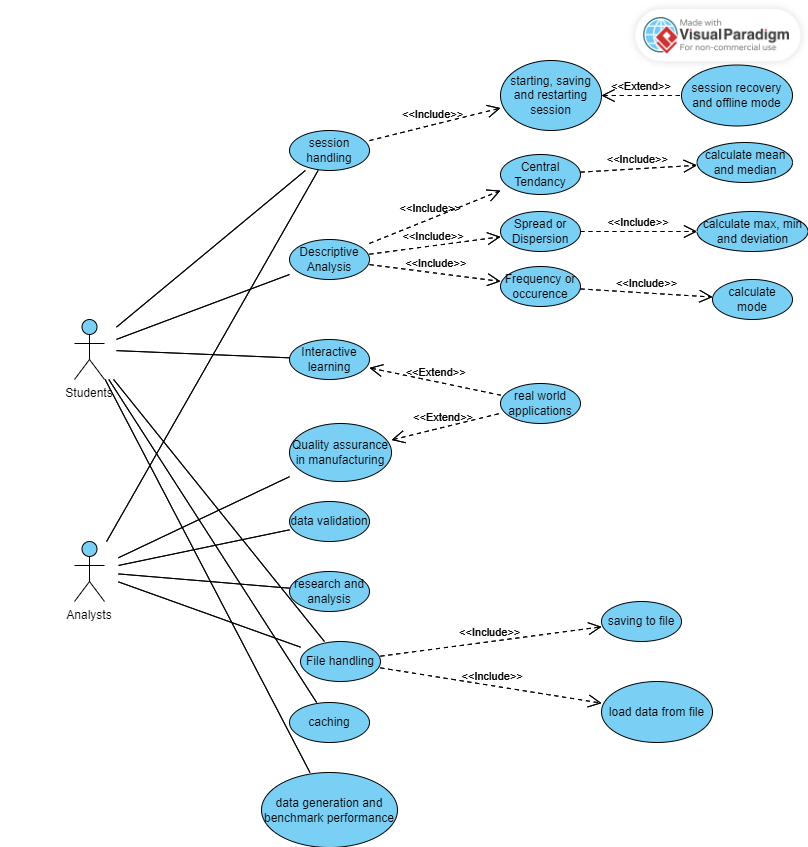
\includegraphics[width=0.75\linewidth]{usecase.png}
    \end{center}
       \caption{Use Case Model \label{Use Case Model}}
\end{figure}

\section{Use Cases}
\subsection{Use Case-1}
\begin{table}[H]
 			\centering
\begin{tabular}{p{1.23in}p{4.87in}}
\hline

%row no:1
\multicolumn{1}{|p{1.23in}}{Use Case ID} & 
\multicolumn{1}{|p{4.87in}|}{UC-1} \\
\hhline{--}
%row no:2
\multicolumn{1}{|p{1.23in}}{Use Case Name} & 
\multicolumn{1}{|p{4.87in}|}{Session handling} \\
\hhline{--}
%row no:3
\multicolumn{1}{|p{1.23in}}{Primary Actors} & 
\multicolumn{1}{|p{4.87in}|}{Student} \\
\hhline{--}
%row no:4
\multicolumn{1}{|p{1.23in}}{Priority} & 
\multicolumn{1}{|p{4.87in}|}{High} \\
\hhline{--}
%row no:5
\multicolumn{1}{|p{1.23in}}{Description} & 
\multicolumn{1}{|p{4.87in}|}{The Session Handling use case is responsible for managing the user sessions within the Metristics system. It ensures that students can securely and efficiently interact with the system while performing statistical calculations on random datasets. } \\
\hhline{--}
%row no:6
\multicolumn{1}{|p{1.23in}}{Pre-conditions} & 
\multicolumn{1}{|p{4.87in}|}{The Metristics system is operational and accessible.The Student (User) has successfully logged into the system } \\
\hhline{--}
%row no:7
\multicolumn{1}{|p{1.23in}}{Post-conditions} & 
\multicolumn{1}{|p{4.87in}|}{The Student (User) can interact with the Metristics system.The session remains active until the Student (User) logs out or becomes inactive for an extended period.} \\
\hhline{--}
%row no:8
\multicolumn{1}{|p{1.23in}}{Normal Flow} & 
\multicolumn{1}{|p{4.87in}|}{\begin{ucmenum}
	\item The Student accesses the Metristics system and provides valid login credentials. \par 	\item The system validates the login credentials and authenticates the Student and logins to system.  \par \item If the Student wishes to log out, system terminates the session, clears session-related data, and returns the Student to the login screen. \par
\end{ucmenum}} \\
\hhline{--}
\end{tabular}
 \end{table}
\subsection{Use Case-2}
\begin{table}[H]
 			\centering
\begin{tabular}{p{1.23in}p{4.87in}}
\hline
%row no:1
\multicolumn{1}{|p{1.23in}}{Use Case ID} & 
\multicolumn{1}{|p{4.87in}|}{UC-2} \\
\hhline{--}
%row no:2
\multicolumn{1}{|p{1.23in}}{Use Case Name} & 
\multicolumn{1}{|p{4.87in}|}{Descriptive analysis} \\
\hhline{--}
%row no:3
\multicolumn{1}{|p{1.23in}}{Primary Actors} & 
\multicolumn{1}{|p{4.87in}|}{Student} \\
\hhline{--}
%row no:4
\multicolumn{1}{|p{1.23in}}{Priority} & 
\multicolumn{1}{|p{4.87in}|}{High} \\
\hhline{--}
%row no:5
\multicolumn{1}{|p{1.23in}}{Description} & 
\multicolumn{1}{|p{4.87in}|}{The Descriptive Analysis use case is responsible for performing statistical analysis on a random dataset within the Metristics system. It calculates essential statistical measures.} \\
\hhline{--}
%row no:6
\multicolumn{1}{|p{1.23in}}{Pre-conditions} & 
\multicolumn{1}{|p{4.87in}|}{The Student has successfully logged into the system. A random dataset is available for analysis} \\
\hhline{--}
%row no:7
\multicolumn{1}{|p{1.23in}}{Post-conditions} & 
\multicolumn{1}{|p{4.87in}|}{The calculated statistical measures are displayed to the Student. The Student can use the generated statistics for further analysis or decision-making. } \\
\hhline{--}
%row no:8
\multicolumn{1}{|p{1.23in}}{Normal Flow} & 
\multicolumn{1}{|p{4.87in}|}{\begin{ucmenum}
	\item The Student logs into the Metristics system and navigates to the Descriptive Analysis feature. \par 	\item The system performs the following statistical calculations.\par \item The system ensures that all calculations are accurate.\par
\end{ucmenum}} \\
\hhline{--}
\end{tabular}
 \end{table}


\subsection{Use Case-3}
\begin{table}[H]
 			\centering
\begin{tabular}{p{1.23in}p{4.87in}}
\hline
%row no:1
\multicolumn{1}{|p{1.23in}}{Use Case ID} & 
\multicolumn{1}{|p{4.87in}|}{UC-3} \\
\hhline{--}
%row no:2
\multicolumn{1}{|p{1.23in}}{Use Case Name} & 
\multicolumn{1}{|p{4.87in}|}{Interactive Learning} \\
\hhline{--}
%row no:3
\multicolumn{1}{|p{1.23in}}{Primary Actors} & 
\multicolumn{1}{|p{4.87in}|}{Student} \\
\hhline{--}
%row no:4
\multicolumn{1}{|p{1.23in}}{Priority} & 
\multicolumn{1}{|p{4.87in}|}{High} \\
\hhline{--}
%row no:5
\multicolumn{1}{|p{1.23in}}{Description} & 
\multicolumn{1}{|p{4.87in}|}{The Interactive Exploration use case within the Metristics system provides Student Analysts with an immersive and interactive environment.\par This use case allows students to interact with practical examples, datasets, and simulations, fostering a deeper understanding of how statistical concepts are applied in real-world scenarios.} \\
\hhline{--}
%row no:6
\multicolumn{1}{|p{1.23in}}{Pre-conditions} & 
\multicolumn{1}{|p{4.87in}|}{The Metristics system is operational and accessible. The Student has successfully logged into the system.} \\
\hhline{--}
%row no:7
\multicolumn{1}{|p{1.23in}}{Post-conditions} & 
\multicolumn{1}{|p{4.87in}|}{Student Analysts have actively engaged in interactive exploration. } \\
\hhline{--}
%row no:8
\multicolumn{1}{|p{1.23in}}{Normal Flow} & 
\multicolumn{1}{|p{4.87in}|}{\begin{ucmenum}
	\item The Student logs into the Metristics system and navigates to the Descriptive Analysis feature.\par 	\item he system provides a rich set of interactive resources and tools.
\end{ucmenum}} \\
\hhline{--}
\end{tabular}
 \end{table}


\subsection{Use Case-4}
\begin{table}[H]
 			\centering
\begin{tabular}{p{1.23in}p{4.87in}}
\hline
%row no:1
\multicolumn{1}{|p{1.23in}}{Use Case ID} & 
\multicolumn{1}{|p{4.87in}|}{UC-4} \\
\hhline{--}
%row no:2
\multicolumn{1}{|p{1.23in}}{Use Case Name} & 
\multicolumn{1}{|p{4.87in}|}{Quality assurance in manufacturing} \\
\hhline{--}
%row no:3
\multicolumn{1}{|p{1.23in}}{Primary Actors} & 
\multicolumn{1}{|p{4.87in}|}{Analysts} \\
\hhline{--}
%row no:4
\multicolumn{1}{|p{1.23in}}{Priority} & 
\multicolumn{1}{|p{4.87in}|}{High} \\
\hhline{--}
%row no:5
\multicolumn{1}{|p{1.23in}}{Description} & 
\multicolumn{1}{|p{4.87in}|}{The Quality Assurance use case within the Metristics system enables Data Analysts to ensure the accuracy, reliability, and quality of statistical analyses and reports generated within the system. It involves a systematic process of reviewing, validating, and verifying analysis results, data integrity, and adherence to best practices and standards.} \\
\hhline{--}
%row no:6
\multicolumn{1}{|p{1.23in}}{Pre-conditions} & 
\multicolumn{1}{|p{4.87in}|}{The Data Analyst has successfully logged into the system. Statistical analyses or reports have been generated.} \\
\hhline{--}
%row no:7
\multicolumn{1}{|p{1.23in}}{Post-conditions} & 
\multicolumn{1}{|p{4.87in}|}{Data Analysts have performed quality assurance checks and ensured the accuracy and reliability of analysis results. QA findings and documentation are available for review and auditing.} \\
\hhline{--}
%row no:8
\multicolumn{1}{|p{1.23in}}{Normal Flow} & 
\multicolumn{1}{|p{4.87in}|}{\begin{ucmenum}
	\item The Data Analyst logs into the Metristics system. \par 	\item The Data Analyst selects the statistical analysis or report that requires quality assurance. \par 	\item The Data Analyst documents their findings, including any issues or concerns identified during the quality assurance process.
\end{ucmenum}} \\
\hhline{--}
\end{tabular}
 \end{table}


\subsection{Use Case-5}
\begin{table}[H]
 			\centering
\begin{tabular}{p{1.23in}p{4.87in}}
\hline
%row no:1
\multicolumn{1}{|p{1.23in}}{Use Case ID} & 
\multicolumn{1}{|p{4.87in}|}{UC-5} \\
\hhline{--}
%row no:2
\multicolumn{1}{|p{1.23in}}{Use Case Name} & 
\multicolumn{1}{|p{4.87in}|}{Data validation} \\
\hhline{--}
%row no:3
\multicolumn{1}{|p{1.23in}}{Primary Actors} & 
\multicolumn{1}{|p{4.87in}|}{Analysts} \\
\hhline{--}
%row no:4
\multicolumn{1}{|p{1.23in}}{Priority} & 
\multicolumn{1}{|p{4.87in}|}{High} \\
\hhline{--}
%row no:5
\multicolumn{1}{|p{1.23in}}{Description} & 
\multicolumn{1}{|p{4.87in}|}{This use case empowers Data Analysts to assess data integrity and suitability for analysis, thereby enhancing the accuracy of statistical results and insights derived from the data.} \\
\hhline{--}
%row no:6
\multicolumn{1}{|p{1.23in}}{Pre-conditions} & 
\multicolumn{1}{|p{4.87in}|}{Data Analysts have successfully logged into the system A dataset is available for validation} \\
\hhline{--}
%row no:7
\multicolumn{1}{|p{1.23in}}{Post-conditions} & 
\multicolumn{1}{|p{4.87in}|}{Data Analysts have verified and validated the dataset for quality and accuracy. Identified data issues or discrepancies are documented and reported. The validated dataset is available for further statistical analysis} \\
\hhline{--}
%row no:8
\multicolumn{1}{|p{1.23in}}{Normal Flow} & 
\multicolumn{1}{|p{4.87in}|}{\begin{ucmenum}
	\item A Data Analyst logs into the Metristics system using their credentials. \par 	\item The system presents the Data Analyst with an option to access the Data Validation module. \par 	\item The Data Analyst selects the dataset they want to validate from a list of available dataset
\end{ucmenum}} \\
\hhline{--}
\end{tabular}
 \end{table}


\subsection{Use Case-6}
\begin{table}[H]
 			\centering
\begin{tabular}{p{1.23in}p{4.87in}}
\hline
%row no:1
\multicolumn{1}{|p{1.23in}}{Use Case ID} & 
\multicolumn{1}{|p{4.87in}|}{UC-6} \\
\hhline{--}
%row no:2
\multicolumn{1}{|p{1.23in}}{Use Case Name} & 
\multicolumn{1}{|p{4.87in}|}{Research and analysis} \\
\hhline{--}
%row no:3
\multicolumn{1}{|p{1.23in}}{Primary Actors} & 
\multicolumn{1}{|p{4.87in}|}{Analysts} \\
\hhline{--}
%row no:4
\multicolumn{1}{|p{1.23in}}{Priority} & 
\multicolumn{1}{|p{4.87in}|}{High} \\
\hhline{--}
%row no:5
\multicolumn{1}{|p{1.23in}}{Description} & 
\multicolumn{1}{|p{4.87in}|}{This use case provides the necessary tools and functionalities for data exploration, hypothesis testing, and statistical modeling, enabling analysts to discover trends, patterns, and correlations within the data.} \\%row no:6
\multicolumn{1}{|p{1.23in}}{Pre-conditions} & 
\multicolumn{1}{|p{4.87in}|}{Data Analysts have successfully logged into the system. A dataset is available for analysis.} \\
\hhline{--}
%row no:7
\multicolumn{1}{|p{1.23in}}{Post-conditions} & 
\multicolumn{1}{|p{4.87in}|}{Data Analysts have conducted research and statistical analysis on the dataset. Insights and findings from the analysis are documented and available for reporting. Statistical results are accurate and reliable for decision-making.} \\ %row no:8
\multicolumn{1}{|p{1.23in}}{Normal Flow} & 
\multicolumn{1}{|p{4.87in}|}{\begin{ucmenum}
	\item A Data Analyst logs into the Metristics system using their credentials. \par 	\item The Data Analyst selects the dataset they want to analyze from a list of available datasets, the Data Analyst will initiate the validation . \par 	\item Once the analysis is complete, the Data Analyst will generate reports.
\end{ucmenum}} \\
\hhline{--}
\end{tabular}
 \end{table}



\subsection{Use Case-7}
\begin{table}[H]
 			\centering
\begin{tabular}{p{1.23in}p{4.87in}}
\hline
%row no:1
\multicolumn{1}{|p{1.23in}}{Use Case ID} & 
\multicolumn{1}{|p{4.87in}|}{UC-7} \\
\hhline{--}
%row no:2
\multicolumn{1}{|p{1.23in}}{Use Case Name} & 
\multicolumn{1}{|p{4.87in}|}{File handling} \\
\hhline{--}
%row no:3
\multicolumn{1}{|p{1.23in}}{Primary Actors} & 
\multicolumn{1}{|p{4.87in}|}{Analysts, Students} \\
\hhline{--}
%row no:4
\multicolumn{1}{|p{1.23in}}{Priority} & 
\multicolumn{1}{|p{4.87in}|}{Medium} \\
\hhline{--}
%row no:5
\multicolumn{1}{|p{1.23in}}{Description} & 
\multicolumn{1}{|p{4.87in}|}{The File Handling use case within the Metristics system allows Data Analysts to save data, reports, and analysis artifacts to files for storage, sharing, or future reference.} \\
\hhline{--}
\multicolumn{1}{|p{1.23in}}{Pre-conditions} & 
\multicolumn{1}{|p{4.87in}|}{Data Analysts and students have successfully logged into the system. Data or analysis artifacts are available for export and file handling} \\
\hhline{--}
%row no:7
\multicolumn{1}{|p{1.23in}}{Post-conditions} & 
\multicolumn{1}{|p{4.87in}|}{Data Analysts and students have successfully saved data or analysis artifacts to files. Saved files are stored in a designated location and are accessible for further use. Data Analysts may share saved files with team members or stakeholders as needed.} \\
\hhline{--}
%row no:8
\multicolumn{1}{|p{1.23in}}{Normal Flow} & 
\multicolumn{1}{|p{4.87in}|}{\begin{ucmenum}
	\item A Data Analyst or student logs into the Metristics system using their credentials. \par 	\item The Data Analyst selects the data or analysis artifacts they want to save to a file. This can include datasets, analysis reports, visualizations, or any other relevant information. \par 	\item The Data Analyst and students confirms the file-saving operation.
\end{ucmenum}} \\
\hhline{--}
\end{tabular}
 \end{table}



\subsection{Use Case-8}
\begin{table}[H]
 			\centering
\begin{tabular}{p{1.23in}p{4.87in}}
\hline
%row no:1
\multicolumn{1}{|p{1.23in}}{Use Case ID} & 
\multicolumn{1}{|p{4.87in}|}{UC-8} \\
\hhline{--}
%row no:2
\multicolumn{1}{|p{1.23in}}{Use Case Name} & 
\multicolumn{1}{|p{4.87in}|}{Caching} \\
\hhline{--}
%row no:3
\multicolumn{1}{|p{1.23in}}{Primary Actors} & 
\multicolumn{1}{|p{4.87in}|}{\begin{itemize}
	\item Analysts
\end{itemize}} \\
\hhline{--}
%row no:4
\multicolumn{1}{|p{1.23in}}{Priority} & 
\multicolumn{1}{|p{4.87in}|}{Medium} \\
\hhline{--}
%row no:5
\multicolumn{1}{|p{1.23in}}{Description} & 
\multicolumn{1}{|p{4.87in}|}{The Caching use case in the Metristics system allows Data Analysts to improve the performance and efficiency of data retrieval and analysis by temporarily storing frequently accessed data or computation results in a cache.} \\
\hhline{--}
%row no:6
\multicolumn{1}{|p{1.23in}}{Pre-conditions} & 
\multicolumn{1}{|p{4.87in}|}{\begin{itemize}
	\item Data Analysts have successfully logged into the system. Data or computation results are available for caching.
\end{itemize}} \\
\hhline{--}
%row no:7
\multicolumn{1}{|p{1.23in}}{Post-conditions} & 
\multicolumn{1}{|p{4.87in}|}{\begin{itemize}
	\item Data Analysts have effectively cached data or computation results. Cached data is available for quick retrieval during subsequent analysis or operations.
\end{itemize}} \\
\hhline{--}
%row no:8
\multicolumn{1}{|p{1.23in}}{Normal Flow} & 
\multicolumn{1}{|p{4.87in}|}{\begin{ucmenum}
	\item A Data Analyst logs into the Metristics system using their credentials.\par 	\item The system presents the Data Analyst with an option to access the Caching module. \par 	\item The Data Analyst selects the data or computation results they want to cache. This can include frequently used datasets, intermediate results of calculations, or other relevant data. \par \item The Data Analyst specifies the cache duration. \par 	\item The Data Analyst confirms the caching operation.
\end{ucmenum}} \\
\hhline{--}
\end{tabular}
 \end{table}


\subsection{Use Case-9}
\begin{table}[H]
 			\centering
\begin{tabular}{p{1.23in}p{4.87in}}
\hline
%row no:1
\multicolumn{1}{|p{1.23in}}{Use Case ID} & 
\multicolumn{1}{|p{4.87in}|}{UC-9} \\
\hhline{--}
%row no:2
\multicolumn{1}{|p{1.23in}}{Use Case Name} & 
\multicolumn{1}{|p{4.87in}|}{Benchmark Performance} \\
\hhline{--}
%row no:3
\multicolumn{1}{|p{1.23in}}{Primary Actors} & 
\multicolumn{1}{|p{4.87in}|}{\begin{itemize}
	\item Analysts
\end{itemize}} \\
\hhline{--}
%row no:4
\multicolumn{1}{|p{1.23in}}{Priority} & 
\multicolumn{1}{|p{4.87in}|}{High} \\
\hhline{--}
%row no:5
\multicolumn{1}{|p{1.23in}}{Description} & 
\multicolumn{1}{|p{4.87in}|}{The Benchmark Performance use case in the Metristics system enables Data Analysts to assess and compare the performance of different statistical models or algorithms when applied to the same dataset. This use case helps analysts identify the most efficient and accurate approach for their specific analysis needs, contributing to data-driven decision-making.} \\
\hhline{--}
%row no:6
\multicolumn{1}{|p{1.23in}}{Pre-conditions} & 
\multicolumn{1}{|p{4.87in}|}{\begin{itemize}
	\item Data Analysts have successfully logged into the system. Multiple statistical models or algorithms are available for benchmarking. A dataset is prepared and ready for benchmarking.
\end{itemize}} \\
\hhline{--}
%row no:7
\multicolumn{1}{|p{1.23in}}{Post-conditions} & 
\multicolumn{1}{|p{4.87in}|}{\begin{itemize}
	\item Data Analysts have benchmarked the performance of different statistical models or algorithms. Comparative results are available for analysis and model selection.
\end{itemize}} \\
\hhline{--}
%row no:8
\multicolumn{1}{|p{1.23in}}{Normal Flow} & 
\multicolumn{1}{|p{4.87in}|}{\begin{ucmenum}
	\item A Data Analyst logs into the Metristics system using their credentials. \par 	\item The Data Analyst configures benchmarking parameters, such as evaluation metrics, validation methods (e.g., cross-validation), and performance criteria (e.g., accuracy, precision, recall). \par 	\item The system validates the benchmarking settings to ensure they comply with system guidelines and requirements.
\end{ucmenum}} \\
\hhline{--}
\end{tabular}
 \end{table}




\begin{thebibliography}{5}
    

\bibitem{GQM approach} 
1.GQM Approach    \\\textit{https://www.cs.umd.edu/users/mvz/handouts/gqm.pdf}.   
\bibitem{Use Case Diagram} 
2. Use Case Diagram.,
\\\texit{https://www.visual-paradigm.com/guide/uml-unified-modeling-language/what is use case diagram/}
\bibitem{GQM}
3. Goal-Question-Metric (GQM) Approach for Software Quality Measurement\parencite{gqm_ref}
\bibitem{GQM}
4. Applying the Goal-Question-Metric (GQM) Framework to Improve Project Management\parencite{gqm_conf}
\bibitem{GQM}
5. Goal-Question-Metric (GQM): A Practical Introduction\parencite{gqm_book}
\bibitem{GQM}
6. A Use Case Study for E-commerce Checkout\parencite{usecase_ref}
\bibitem{GQM}
7. Enhancing User Experience: A Mobile Banking Use Case\parencite{usecase_conf}
\bibitem{GQM}
8. Use Cases in Software Engineering\parencite{usecase_book}
\end{thebibliography}

\end{document}
